%%%%%%%%%%%%%%%%%%%%%%%%%%%%%%%%%%%%%%%%%%%%%%%%%%%%%%%%%%%
% --------------------------------------------------------
% Tau
% LaTeX Template
% Version 2.4.3 (01/09/2024)
%
% Author: 
% Guillermo Jimenez (memo.notess1@gmail.com)
% 
% License:
% Creative Commons CC BY 4.0
% --------------------------------------------------------
%%%%%%%%%%%%%%%%%%%%%%%%%%%%%%%%%%%%%%%%%%%%%%%%%%%%%%%%%%%

\documentclass[9pt,a4paper,twoside]{tau-class/tau}
\usepackage[english]{babel}

%----------------------------------------------------------
% TITLE
%----------------------------------------------------------

\journalname{Aprenentatge Computacional}
%% TODO: Optional, you can set a fancier title if you like
\title{Classificació de Supervivents del Titanic}

%----------------------------------------------------------
% AUTHORS, AFFILIATIONS AND PROFESSOR
%----------------------------------------------------------

%% TODO: Set your names here
\author[a,1]{Ricard Urpí Vilanova}
\author[b,2]{Ferran Villarta}
\author[c,3]{Natan Sisoev}

%----------------------------------------------------------

\affil[a]{1711326}
\affil[b]{1704051}
\affil[c]{1706198}

%----------------------------------------------------------
% FOOTER INFORMATION
%----------------------------------------------------------

\institution{Universitat Autònoma de Barcelona}
\footinfo{Pràctica Guiada}
\theday{\today}
\leadauthor{Group GPA-1} 		%% TODO: Set your group ID here
\course{Aprenentatge Computacional}

%----------------------------------------------------------
% ABSTRACT AND KEYWORDS
%----------------------------------------------------------

\begin{abstract}    
	%% TODO: Change this default abstract into something nice that describes your work.
	%% Keep it below 300 words.
    An abstract is a brief summary that outlines the key aspects of a work. An example of a famous abstract is reproduced verbatim here for illustration purposes \cite{vaswani_attention_2017}: The dominant sequence transduction models are based on complex recurrent or convolutional neural networks that include an encoder and a decoder. The best performing models also connect the encoder and decoder through an attention mechanism. We propose a new simple network architecture, the Transformer, based solely on attention mechanisms, dispensing with recurrence and convolutions entirely. Experiments on two machine translation tasks show these models to be superior in quality while being more parallelizable and requiring significantly less time to train. Our model achieves 28.4 BLEU on the WMT 2014 Englishto-German translation task, improving over the existing best results.
\end{abstract}

%----------------------------------------------------------

%% TODO: Set appropriate keywords for your report.
\keywords{a, b, c, d}

%----------------------------------------------------------

\begin{document}
	%% Do NOT change any of this. Line numbers should be kept.
    \maketitle 
    \thispagestyle{firststyle} \tauabstract 
    \tableofcontents
    \linenumbers 
    
%----------------------------------------------------------

\section{EDA (exploratory data analysis)}

Llegint i analitzant la base de dades vam veure que teniem les següents variables:

\begin{itemize}
    \item \textbf{PassengerId}: etiqueta, identifica a cada persona
    \item \textbf{Survived}: binària, 1 = sí, 0 = no
    \item \textbf{Pclass}: categòrica, 1 = primera, 2 = segona, 3 = tercera classe
    \item \textbf{Name}: etiqueta, nom de la persona (potser no únic)
    \item \textbf{Sex}: categòrica, female o male
    \item \textbf{Age}: numèrica, edat en anys
    \item \textbf{SibSp}: numèrica, nombre de germans o parelles en el Titanic
    \item \textbf{Parch}: numèrica, nombre de pares o fills en el Titanic
    \item \textbf{Ticket}: text, codi del tiquet
    \item \textbf{Fare}: numèrica, preu del tiquet
    \item \textbf{Cabin}: text, codi de la cabina
    \item \textbf{Embarked}: categòrica, port d'embarcació: C = Cherbourg, Q = Queenstown, S = Southampton
\end{itemize}

El target és l'atribut \textbf{Survived}, que pot prendre valors 0 o 1.

Ens faltaven dades, el port d'embarcació per a 2 persones, l'edat per a 177 i la cabina per a 687.

Analitzant les correlacions entre variables i la distribució de les dades no trobem grans inconvenients i ens cal acabar de seleccionar, normalitzar i processar les dades.

\begin{figure}[H]
    \centering
    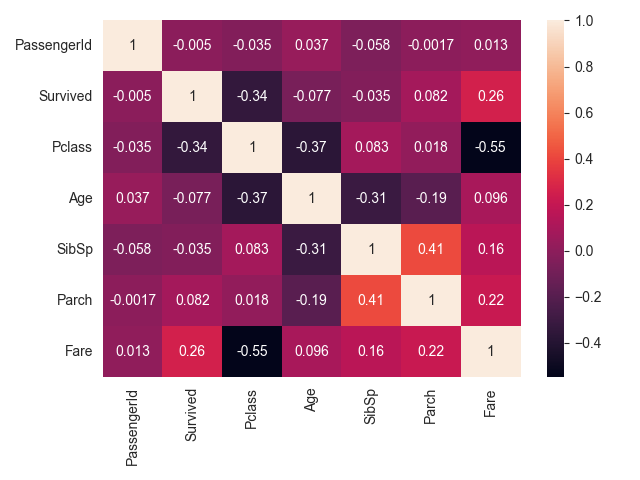
\includegraphics[width=0.4\textwidth]{figures/matriu_corr.png}
    \caption{Matriu de correlacions}
    \label{fig:exemple}
\end{figure}

\section{Preprocessing}

Per a tractar les dades que ens falten hem començat per la cabina, considerem que és molt important per a la predicció, ho podem veure en la següent forografía.

\begin{figure}[H]
    \centering
    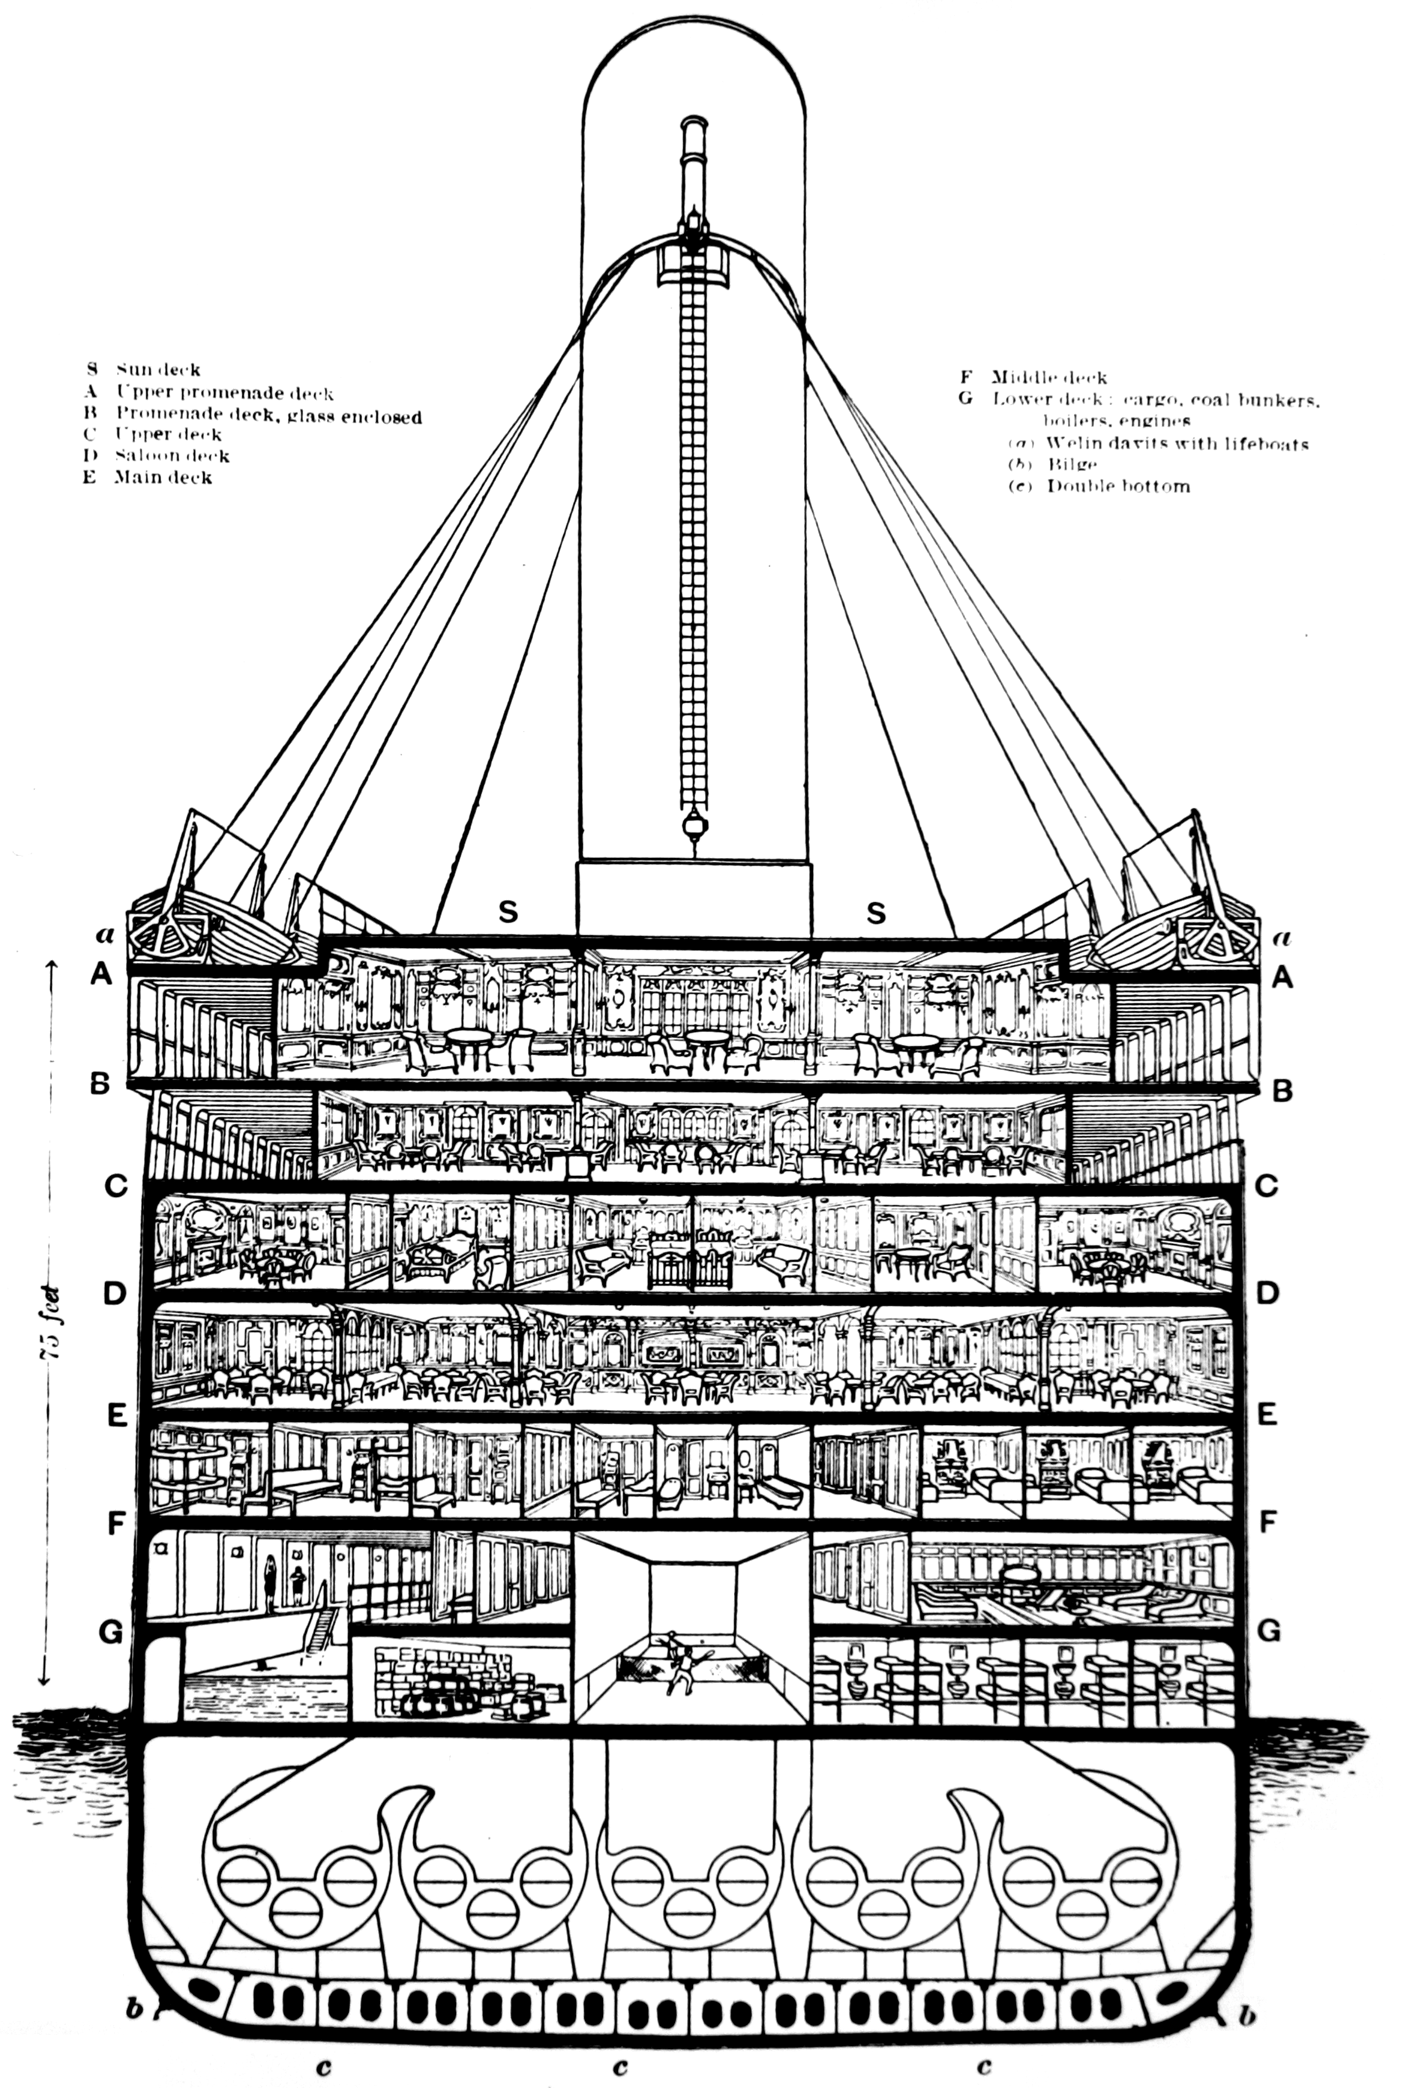
\includegraphics[width=0.2\textwidth]{figures/decks.png}
    \caption{Decks}
    \label{fig:exemple}
\end{figure}


Com ens falten moltes dades (aproximadament 80\% dels passatgers no tenen cabina) no té sentit assignar una cabina a cada passatger, hem creat una nova variable que conté la lletra del codi de la cabina i els passatgers que no en tenen els hem assignat una X. Afegim una variable que indica si tenen cabina o no.
Als passatgers que no tenien port hem considerat que podíem mirar passatgers que tinguin preus de tíquets similars i assignar a aquests passatgers aquest port.
En el cas de l'edat hem decidit imputar les dades que ens falten (20\% aproximadament), la mitjana d'edat varia molt entre classes, les classes més pobres tenen una mitjana d'edat menor així que hem creat una variable que ens indica el nombre de familiars (més familiars pot indicar una edat més baixa), a més a més, tots els noms tenen un títol i aquests corresponen majoritàriament a una certa franja d'edat, sexe...
Hem creat una variable amb el títol de cada persona, creiem que amb aquestes és un bon moment per usar KNN per a trobar passatgers similars i poder assignar una edat als que no en tenim dades, considerem que les variables rellevants són \textbf{Fare}, \textbf{SibSp}, \textbf{Parch}, \textbf{FamilySize}, \textbf{Title}, \textbf{Cabin\_missing} i  \textbf{Pclass}.
Afegim variables binàries per indicar el deck (coberta que correspon a la lletra del codi del tíquet), el port d'embarcament i el sexe.
Finalment, tractem amb els outliers i normalitzem les dades.
El nostre dataset ens queda amb les següents variables ja normalitzades: \textbf{Sex\_male}, \textbf{Embarked\_Q}, \textbf{Embarked\_S}, \textbf{Deck\_B}, \textbf{Deck\_C}, \textbf{Deck\_D},
\textbf{Deck\_E}, \textbf{Deck\_F}, \textbf{Deck\_G}, \textbf{Deck\_X}, \textbf{Title\_Military}, \textbf{Title\_Mr},
\textbf{Title\_Mrs}, \textbf{Title\_Ms}, \textbf{Title\_Nobility}, \textbf{Title\_Rev}, \textbf{Age}, \textbf{SibSp},
\textbf{Parch}, \textbf{Fare}, \textbf{FamilySize}, \textbf{Pclass}, \textbf{PassengerId}, \textbf{Survived} i
\textbf{Cabin\_missing}.

\section{Metric selection}

En aquest apartat hem seleccionat la mètrica que millor s'ajusta al nostre model.
\\\\
Entrenem el model utilitzant regressió logística i obtenim les següents conclusions:

\begin{itemize}

\item \textbf{1. Accuracy}: Pot ser enganyosa en datasets desequilibrats.
   Encara que no és extremadament desequilibrat, hi ha més morts que supervivents.
   Així que un model que prediu gairebé sempre "mor" tindria bona accuracy, però no seria bo per detectar supervivents.

\item \textbf{2. Precision i Recall}: Precision mira quants  supervivents predits realment sobreviuen (minimitza falsos positius).
\\ Recall mira quants  supervivents reals hem detectat (minimitza falsos negatius).
\\Per comparar models cal un equilibri entre ambdues.

\item \textbf{3. Average Precision Score}: Resumeix tota la Precision-Recall curve.
   És útil quan el model retorna probabilitats i hi ha molts casos positius escassos.
   En aquest cas les classes no són extremadament desequilibrades.

\item \textbf{4. ROC-AUC}: També resumeix la capacitat del model per separar classes.
   Però dona menys informació en casos desequilibrats, pot donar una falsa sensació de bon rendiment quan hi ha molts negatius.

\item \textbf{5. F1-score}: Combina Precision i Recall en una mitjana, equilibrant la capacitat de detectar supervivents (recall) i no predir falsament supervivents (precision).

\end{itemize}

Per aquests motius, hem triat l'F1-score com a mètrica principal per avaluar els models.

\begin{figure}[H]
    \centering
    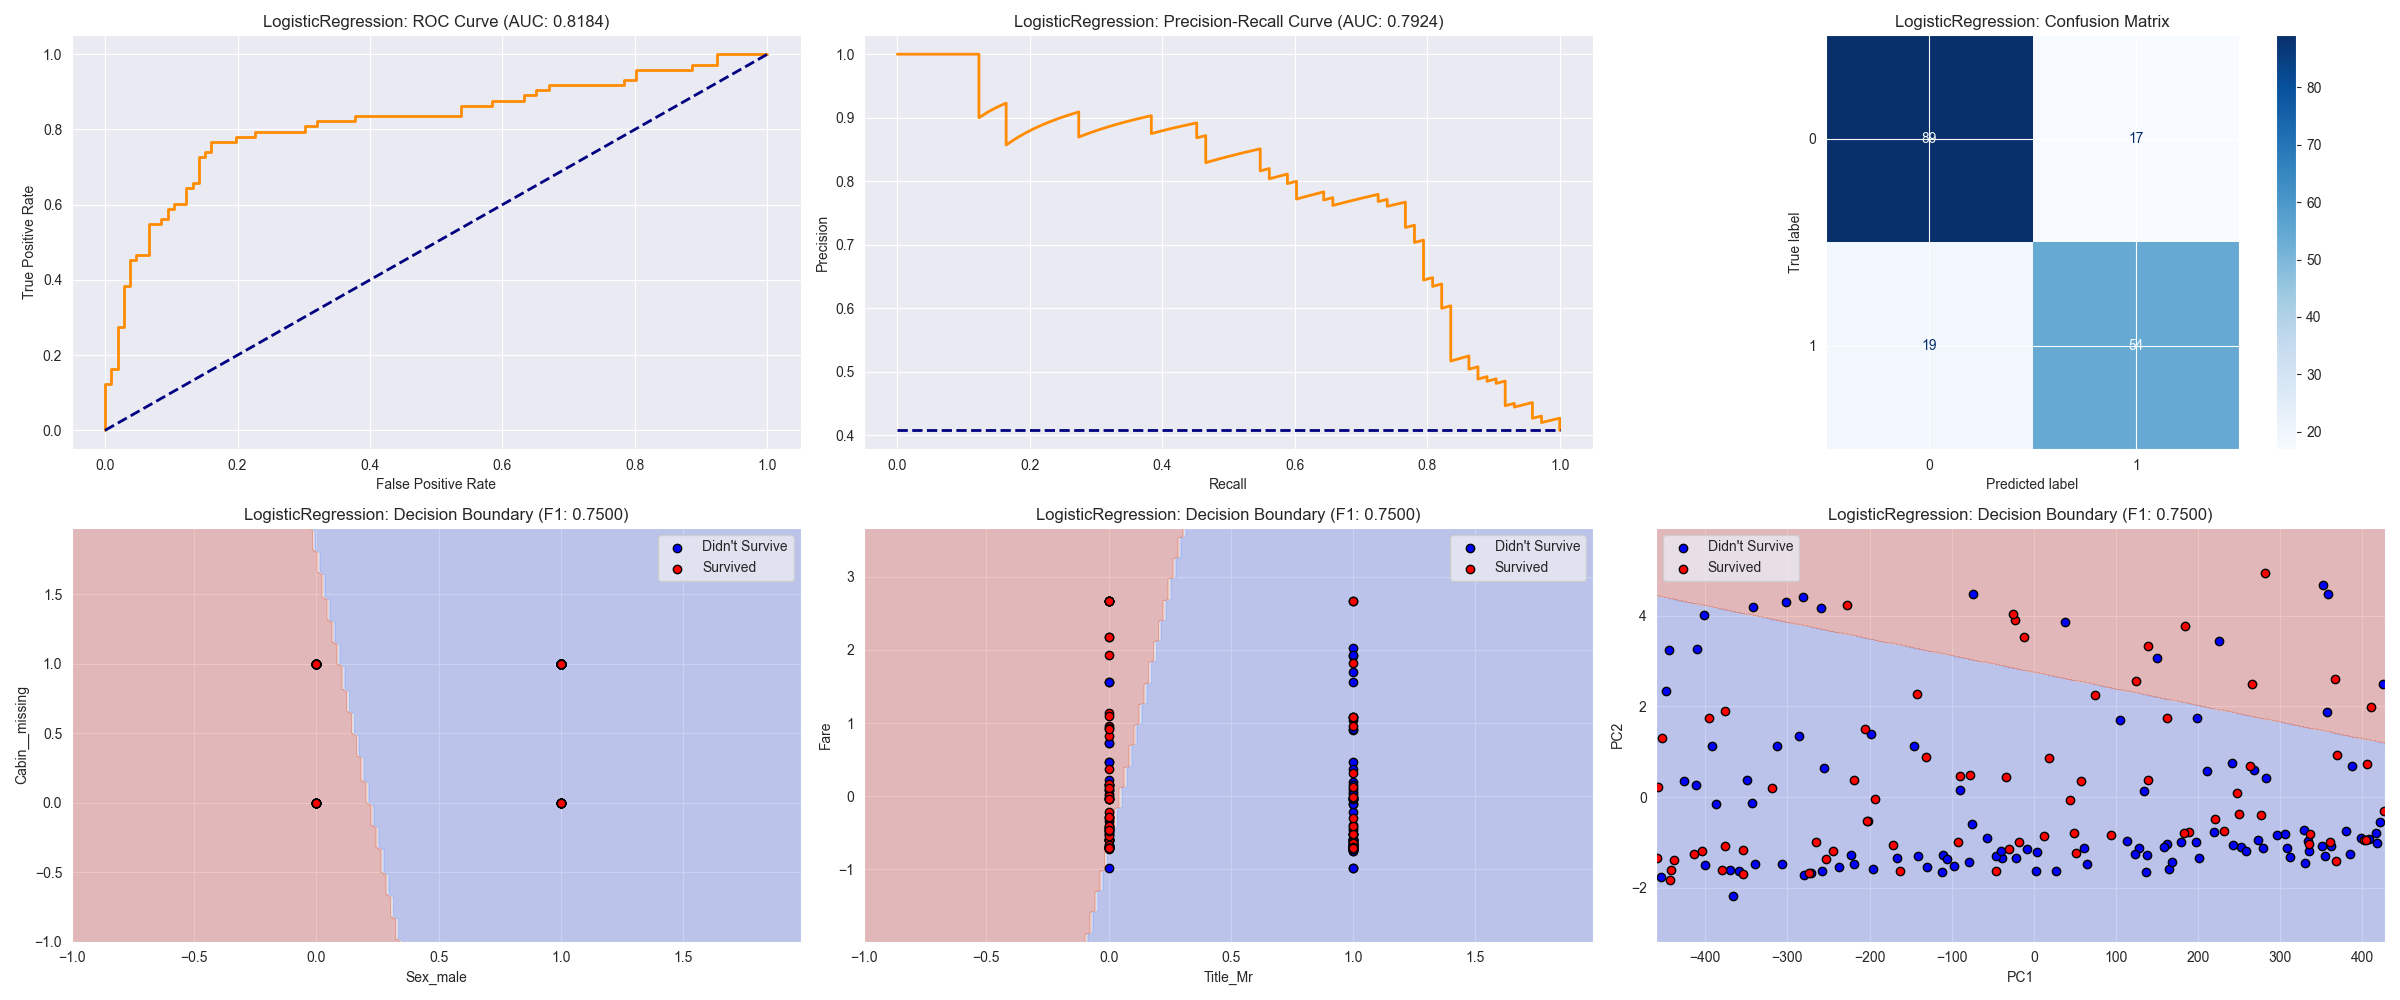
\includegraphics[width=0.4\textwidth]{figures/punt3.png}
    \caption{Gràfics}
    \label{fig:exemple}
\end{figure}

Podem observar com hem generat diferents gràfics representant les dues corbes, la matriu de confusió, les fronteres per dues parelles de features i PCA.

\section{Model Selection amb Crossvalidation}

Els mètodes que hem provat per fer validació creuada han estat: K-Fold, Stratified K-Fold, Repeated Stratified K-Fold i Shuffle \& Split. Els hem provat tots amb cadascun dels mètodes que presentarem a continuació. Com és un dataset petit, hem decidit escollir el més reobust, tot i tardar una mica més: Repeated Stratified K-Fold. L'implementem directament en la nostra class \texttt{Metrics}, de manera que qualsevol testeig que fem serà fent servir aquest tipus de validació creuada.

Seleccionem els següents models:
\begin{itemize}
    \item \textbf{Logistic Regression}
    \item \textbf{KNN}
    \item \textbf{Gradient Descent}
    \item \textbf{Random Forest}
    \item \textbf{Extra Trees}
    \item \textbf{Support Vector Machine}
    \item \textbf{LinearSVC}
    \item \textbf{Gradient Boosting}
    \item \textbf{Naive Bayes}
    \item \textbf{Perceptron}
    \item \textbf{Passive Agressive}
    \item \textbf{Neural Network}
\end{itemize}

Els més adequats són Random Forest, Extra Trees i Gradient Boosting, que gestionen bé petites mostres i desequilibris. Models lineals com Logistic Regression i SVC poden funcionar si les dades estan normalitzades, mentre que Perceptron i Passive Aggressive són menys útils. Altres com KNN, Naive Bayes o MLPClassifier poden donar resultats raonables però requereixen cura amb hiperparàmetres o tenen risc d’overfit.

Hem provat a reduïr la dimensionalitat del model per a veure si obtenim bons resultats en dimensions menor que poguem visualitzar, aquests són alguns dels resultats que hem obtingut:

\begin{figure}[H]
    \centering
    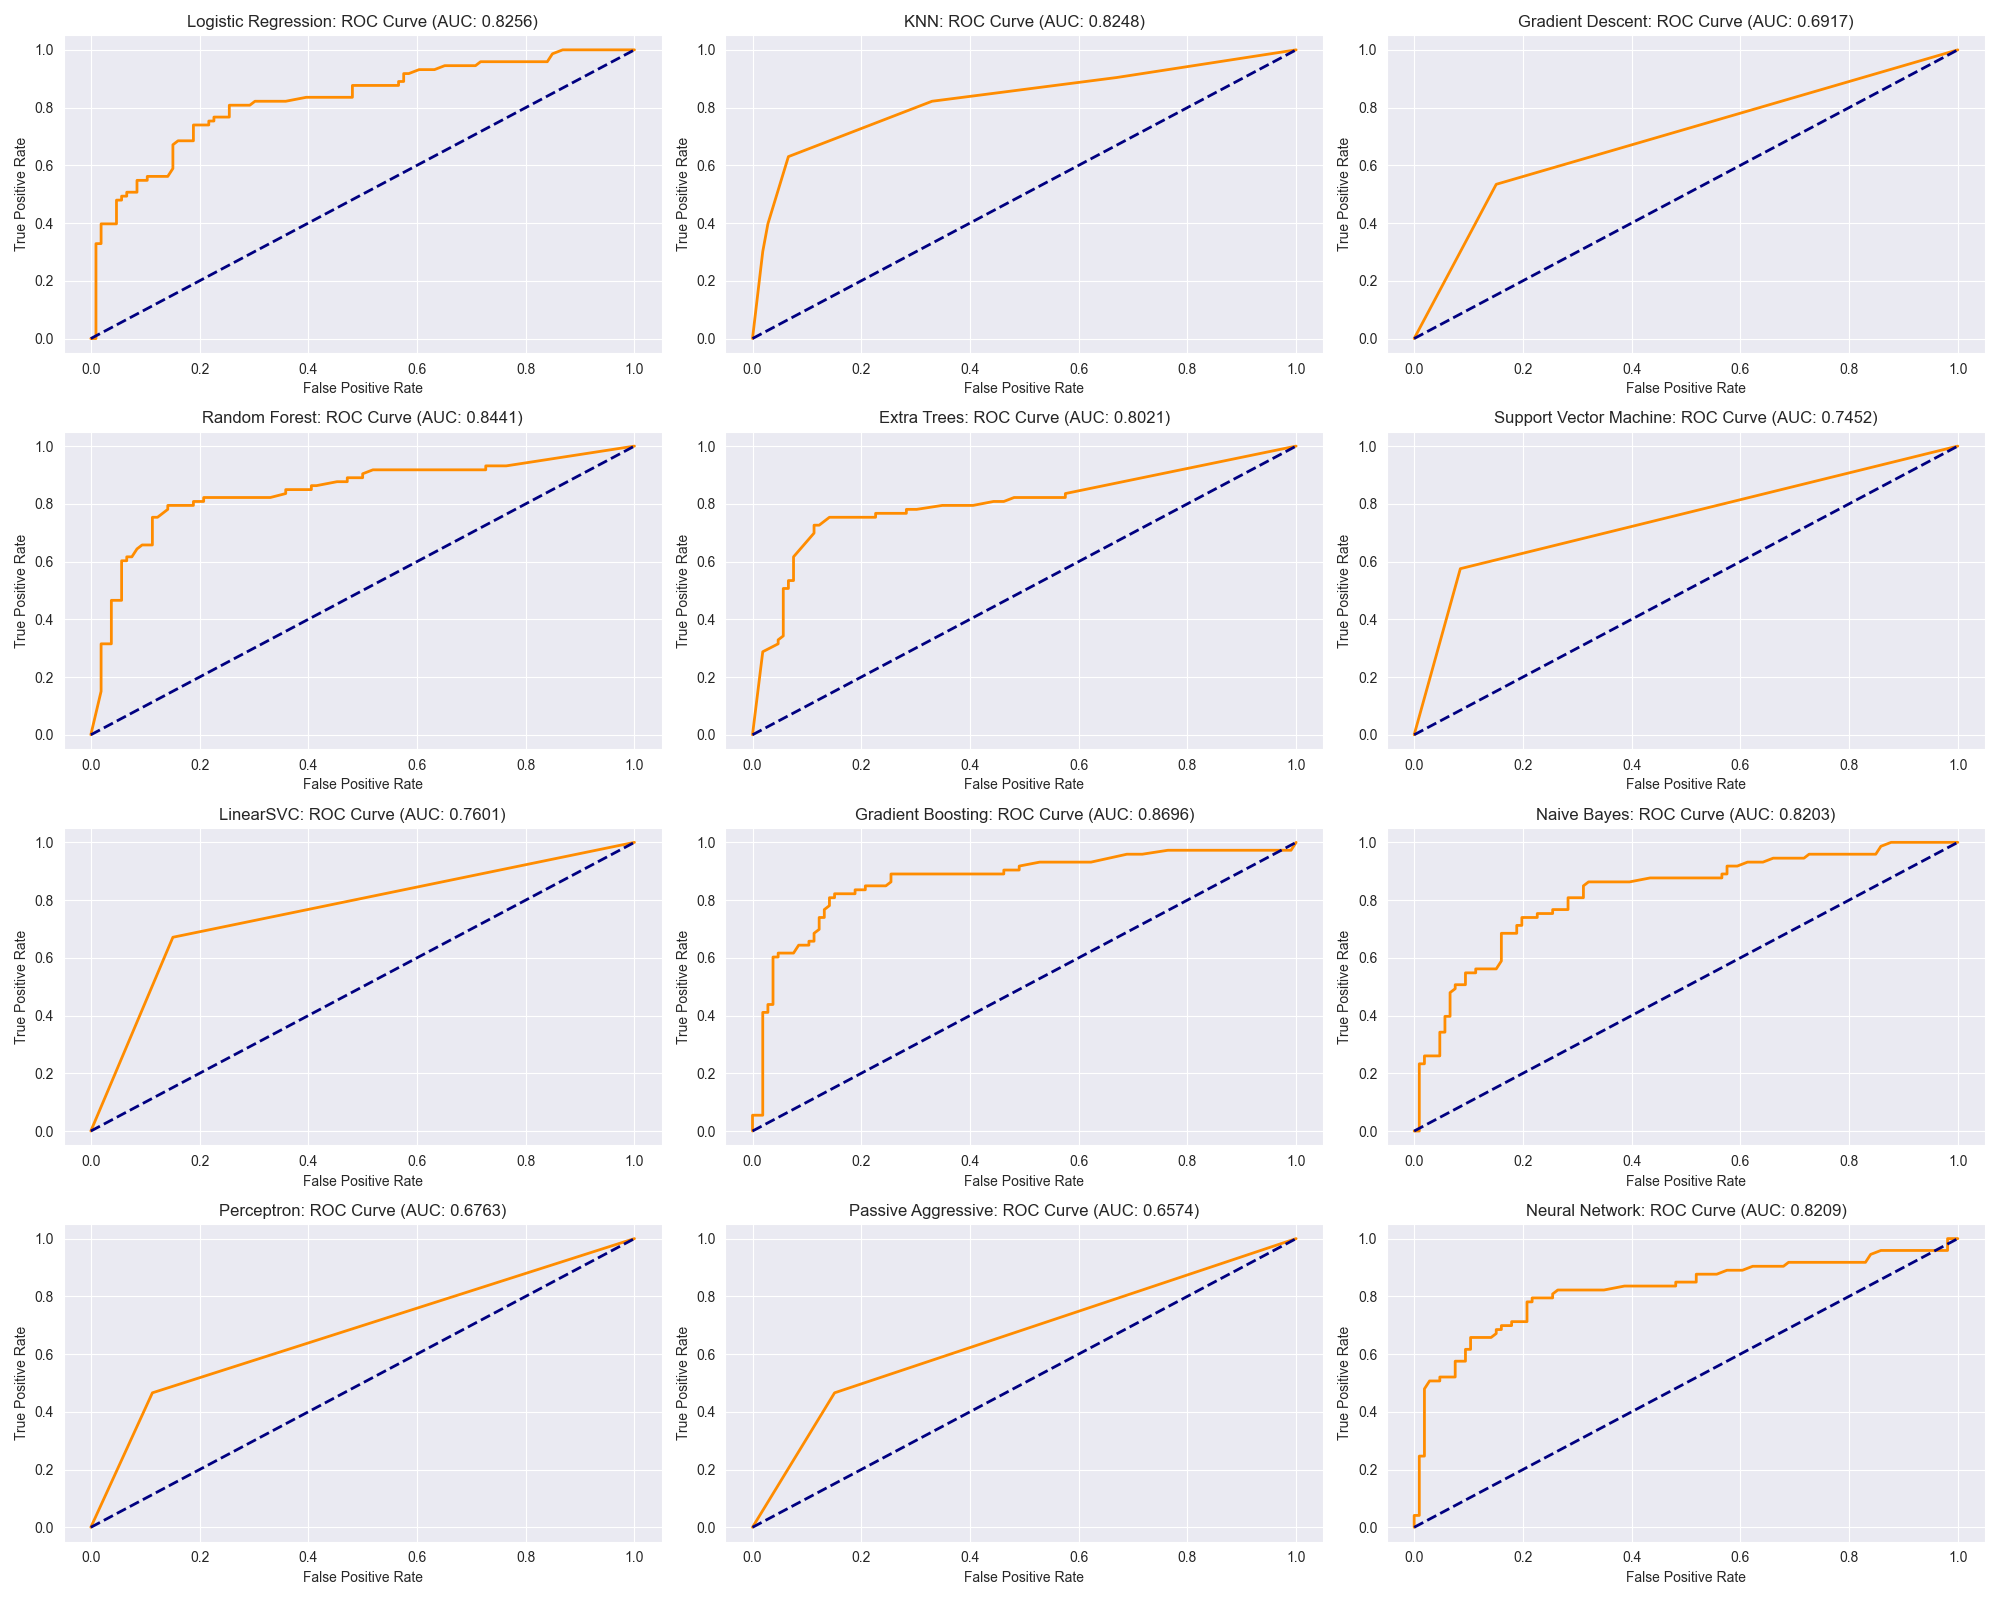
\includegraphics[width=0.4\textwidth]{figures/red_dims.png}
    \caption{Corbes amb el dataset reduït}
    \label{fig:exemple}
\end{figure}

\section{Anàlisi Final}
\textbf{RESULTATS DEL MODEL TRIAT AMB ELS MILLORS HIPERPARAMETRES}

**Preguntes:**
* Mostreu les corves ROC/PR (la que hagueu escollit en l'apartat 2) i interpreteu els resultats.

* Analitzeu en detall les diferents mètriques que trobeu adients i comenteu per sobre com podrieu fer servir aquest model en un futur. Això és el que es coneix com un cas d'ús.

* Com creieu que es podria millorar el vostre model?


\end{document}